\documentclass{beamer}

\usepackage[brazilian]{babel}
\usepackage[utf8]{inputenc}
\usepackage{graphicx}

\usetheme{default}

\title{\textbf{\Huge G3P}}
\subtitle{Gestor de Parceiros Produtos e Pedidos}
\author{
    Dirley Rodrigues Lima da Silva - 1112130033 \\
    Humberto Rocha Gonçalves Filho - 1112130017
}
\date{\today}


\begin{document}
% Titulo da apresentação
\frame{\titlepage}

% Slide com a descrição do projeto
\begin{frame}
  \frametitle{Descrição}
  \begin{columns}[T]
    \begin{column}{.5\textwidth}
      \begin{itemize}
        \itemsep 1em
        \item Aplicativo
        \item Produtos
        \item Parceiros
        \item Pedidos
      \end{itemize}
    \end{column}
    \begin{column}{.5\textwidth}
      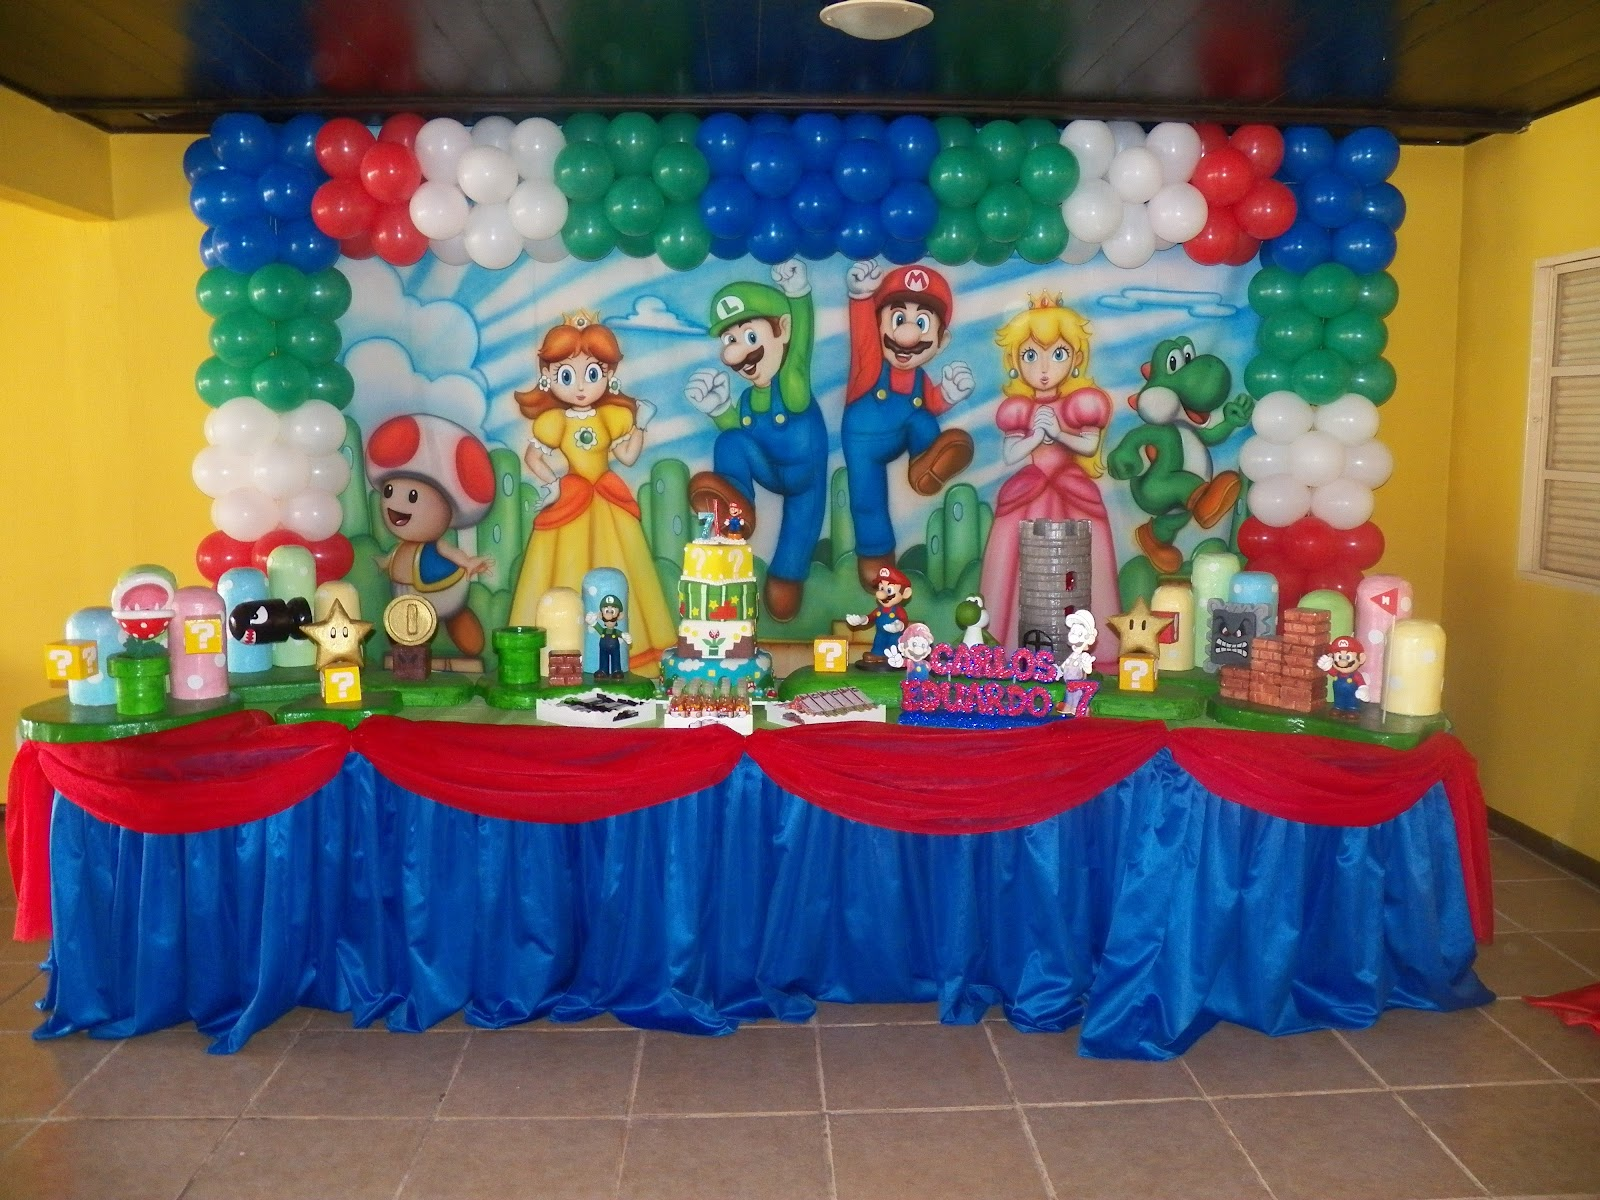
\includegraphics[width=\textwidth]{festa.jpg}
    \end{column}
  \end{columns}
\end{frame}

% Slide com a motivação do projeto
\begin{frame}
  \frametitle{Motivação}
  \begin{itemize}
    \itemsep 1em
    \item Gestão manual
    \item Ausência de padronização
    \item Inconsistências
    \item Ausência de histórico
  \end{itemize}
\end{frame}

% Slide com a proposta de solução
\begin{frame}
  \frametitle{Proposta}
  \begin{columns}[T]
    \begin{column}{.5\textwidth}
      \begin{itemize}
        \itemsep 1em
        \item Catalogar
        \item Padronizar
        \item Automatizar
        \item Centralizar
      \end{itemize}
    \end{column}
    \begin{column}{.5\textwidth}
      
\includegraphics[width=\textwidth]{proposta.jpg}
    \end{column}
  \end{columns}
\end{frame}

% Slide com a modelagem
\begin{frame}
  \frametitle{Conceito}
  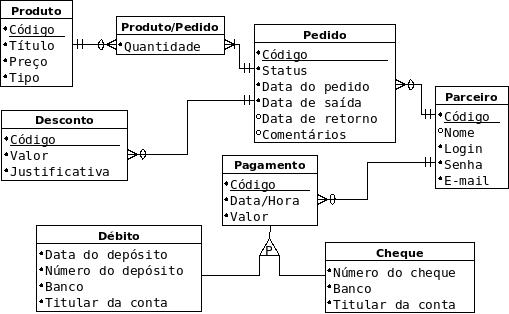
\includegraphics[width=\textwidth]{modelagem.jpg}
\end{frame}

% Slide com as tecnologias usadas
\begin{frame}
  \frametitle{Tecnologias}
  
\includegraphics[width=.5\textwidth]{django.png}
  
\includegraphics[width=.5\textwidth]{python.png}
  
  \centerline{
    \includegraphics[width=.5\textwidth]{sqlite.png}
    
\includegraphics[width=.5\textwidth]{github.jpg}
  }
\end{frame}

% Slide com a arquitetura do django
\begin{frame}
  \frametitle{Aquitetura do django}
  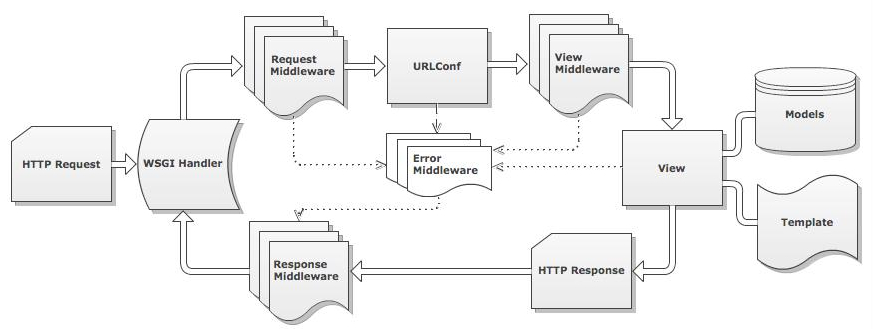
\includegraphics[width=\textwidth]{arquitetura.jpg}
\end{frame}

% Slide com os detalhes de implementação
\begin{frame}
  \frametitle{Implementação}
  \begin{columns}[T]
    \begin{column}{.5\textwidth}
      \begin{block}{Problemas}
        \begin{itemize}
          \itemsep 1em
          \item Histórico
          \item ``Auto incremento''
          \item Limitações do orm
        \end{itemize}
      \end{block}
      \begin{block}{Soluções}
        \begin{itemize}
          \item Versionamento
          \item uuid
          \item Chave Surrogada
        \end{itemize}
      \end{block}
    \end{column}
    \begin{column}{.5\textwidth}
      
\includegraphics[width=\textwidth]{implementacao.jpg}
    \end{column}
  \end{columns}
\end{frame}

% Slide com os agradecimentos
\begin{frame}
  \frametitle{Agradecimentos}
  \begin{center}
    \textbf{\LARGE
      Obrigado!
    }

    
\includegraphics[width=.3\textwidth]{repo.jpg}

    https://github.com/humrochagf/G3P
  \end{center}
\end{frame}

\end{document}